% ============================================================
%  phi(30,2) = phi(30,1) - phi(10,1)      (p_2 = 3)
%  The grid has floor(30/3) = 10 columns, so its first row
%  is exactly the range 1..10 of the subtracted term.
%  Compile with pdflatex.
% ============================================================
\documentclass[border=10pt]{standalone}
\usepackage{tikz}
\usepackage{amsmath}

\newcommand{\figscale}{1.5}   % uniform scale of the whole figure
\newcommand{\cellpitch}{1.2}

\tikzset{
  cell/.style   = {draw, rounded corners=1.5pt, minimum size=0.72cm,
                   inner sep=0pt, font=\small},
  alive/.style  = {fill=green!16,  draw=green!55!black},
  killed/.style = {fill=orange!60, draw=orange!75!black, font=\small\bfseries},
  gone/.style   = {fill=black!5,   draw=black!18, text=black!35},
  fac/.style    = {font=\scriptsize, inner sep=1.5pt, text=blue!65!black,
                   anchor=south east},
}

% \pcell{<cols>}{<n>}{<style>}  -- row-major placement, node named c<n>
\newcommand{\pcell}[3]{%
  \pgfmathsetmacro{\cx}{mod(#2-1,#1)*\cellpitch}%
  \pgfmathsetmacro{\cy}{-floor((#2-1)/#1)*\cellpitch}%
  \node[cell,#3] (c#2) at (\cx,\cy) {#2};%
}
\newcommand{\drawset}[3]{{\edef\phlist{#2}%
  \foreach \n in \phlist {\pcell{#1}{\n}{#3}}}}

\begin{document}
\scalebox{\figscale}{%
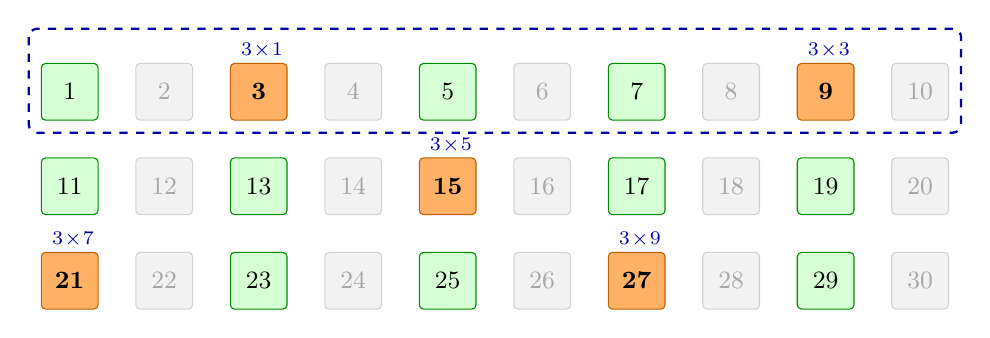
\begin{tikzpicture}

% ---------------- the single table (10 columns) --------------
\drawset{10}{1,5,7,11,13,17,19,23,25,29}{alive}          % phi(30,2)
\drawset{10}{3,9,15,21,27}{killed}                       % removed now
\drawset{10}{2,4,6,8,10,12,14,16,18,20,22,24,26,28,30}{gone}

% ---------------- first row = range of phi(10,1) -------------
\draw[blue!65!black, dashed, thick, rounded corners=3pt]
  (-0.52,0.80) rectangle (11.32,-0.52);

% ---------------- each removed number as  3 x k  --------------
\foreach \n/\k in {3/1, 9/3, 15/5, 21/7, 27/9}{%
  \node[fac] at (c\n.north east) {$3\!\times\!\k$};}

\end{tikzpicture}%
}
\end{document}
